\chapter{Method} \label{ch:method}

We take on the following task: given a dataset of images of weathered cars,
learn a model that generates materials to approximate the appearance of
weathering on a car surface. We focus on Lambertian materials in this thesis and represent the material with a
semi-transparent albedo texture-map in the UV-embedding of the surface.

\begin{figure}[ht]
    \centering
    \caption{Our model pipeline takes as input a scene description $\Phi$ which contains:
        shape geometry, shading materials, camera parameters, and lighting parameters.
        The UV-embedding of the car triangle-mesh, allows us to extract the \emph{position}
        and \emph{normal} maps of the car in its UV-coordinates, which we refer to as the
        \emph{geometry buffer}. The \emph{geometry buffer} is used to generate the albedo
        of the dirt using our generator network $\mathcal{G}$. To produce the final render,
        we use a differentiable ray tracer $\mathcal{R}$ after compositing the dirt albedo
        onto the original shading material.}
    \label{fig:generator-pipeline}
    \vspace{0.2in}
    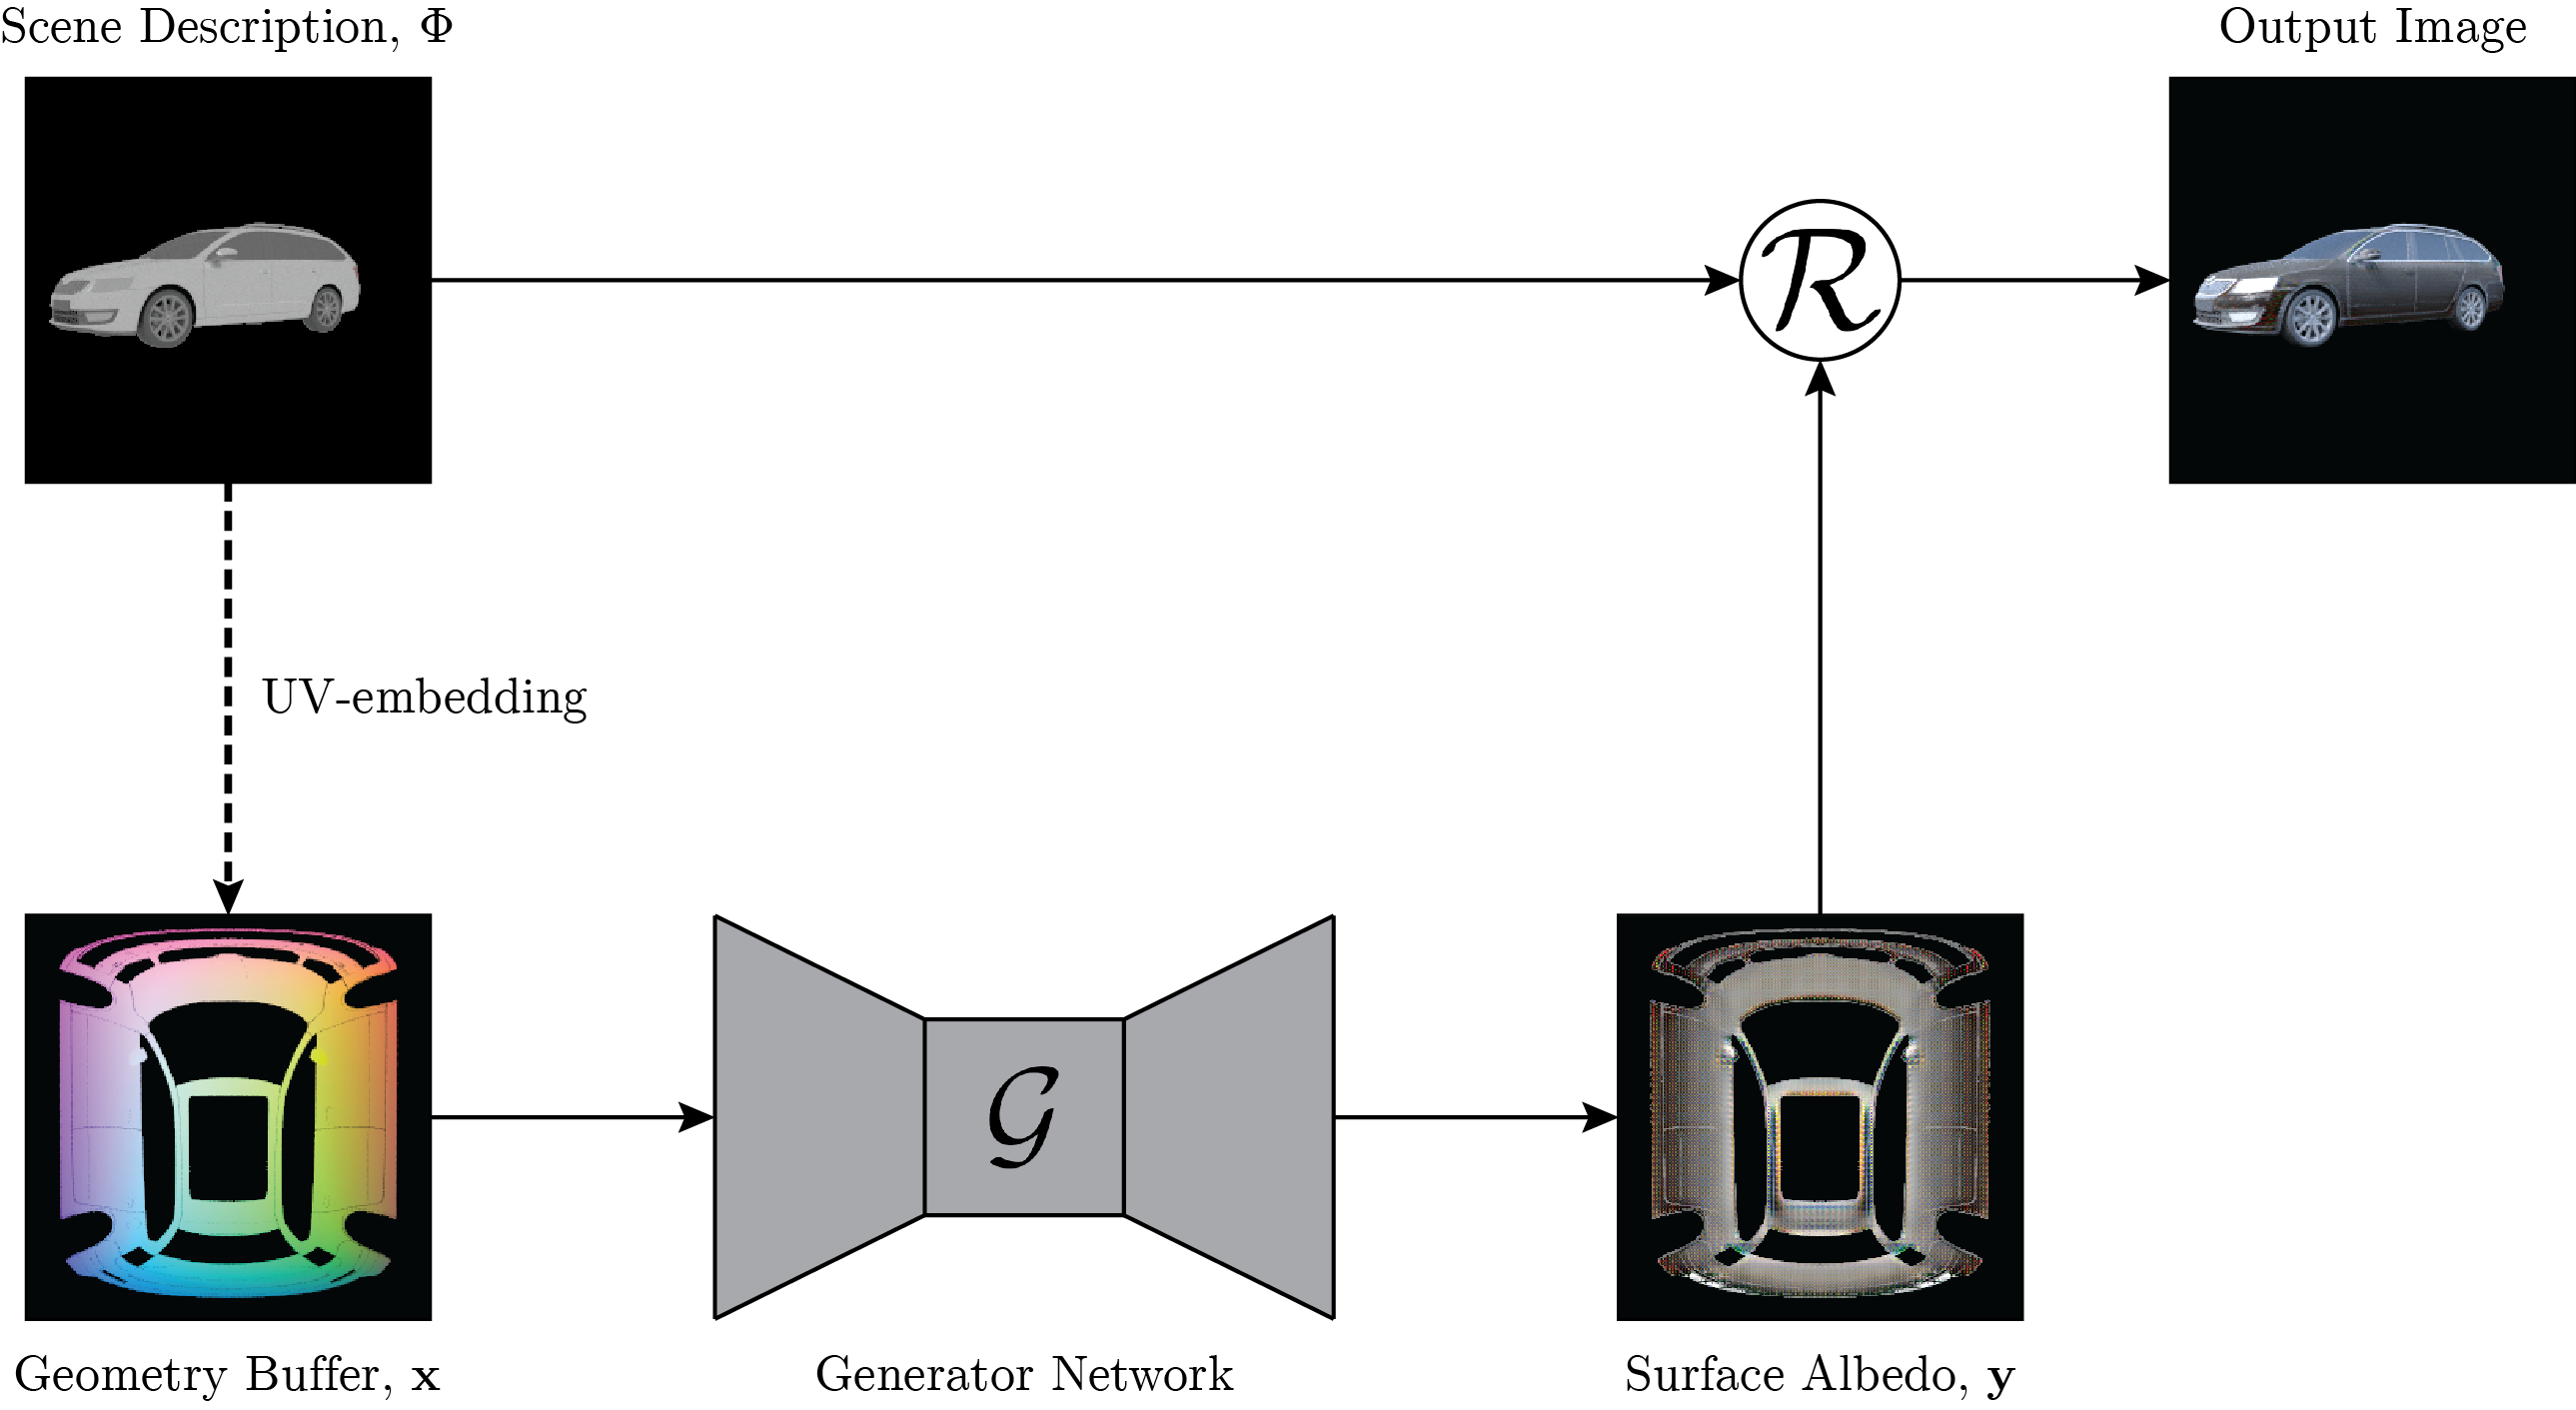
\includegraphics[width=.9\linewidth]{graphics/pipeline.png}
\end{figure}
\begin{figure}[ht]
    \centering
    \caption{We use a GAN training procedure for our model. In addition to our generator model $\mathcal{G}$, we
    train a discriminator model $\mathcal{D}$ that learns to discriminate whether an image was produced by the
    generator (fake) or was sampled from the dataset (real). The discriminator produces a down-sampled grid of
    the input image, with each pixel representing the likelihood of the input being real or fake. In the
    visualization below, the correspondence is: yellow -- real, cyan -- fake.}
    \label{fig:discriminator-pipeline}
    \vspace{0.2in}
    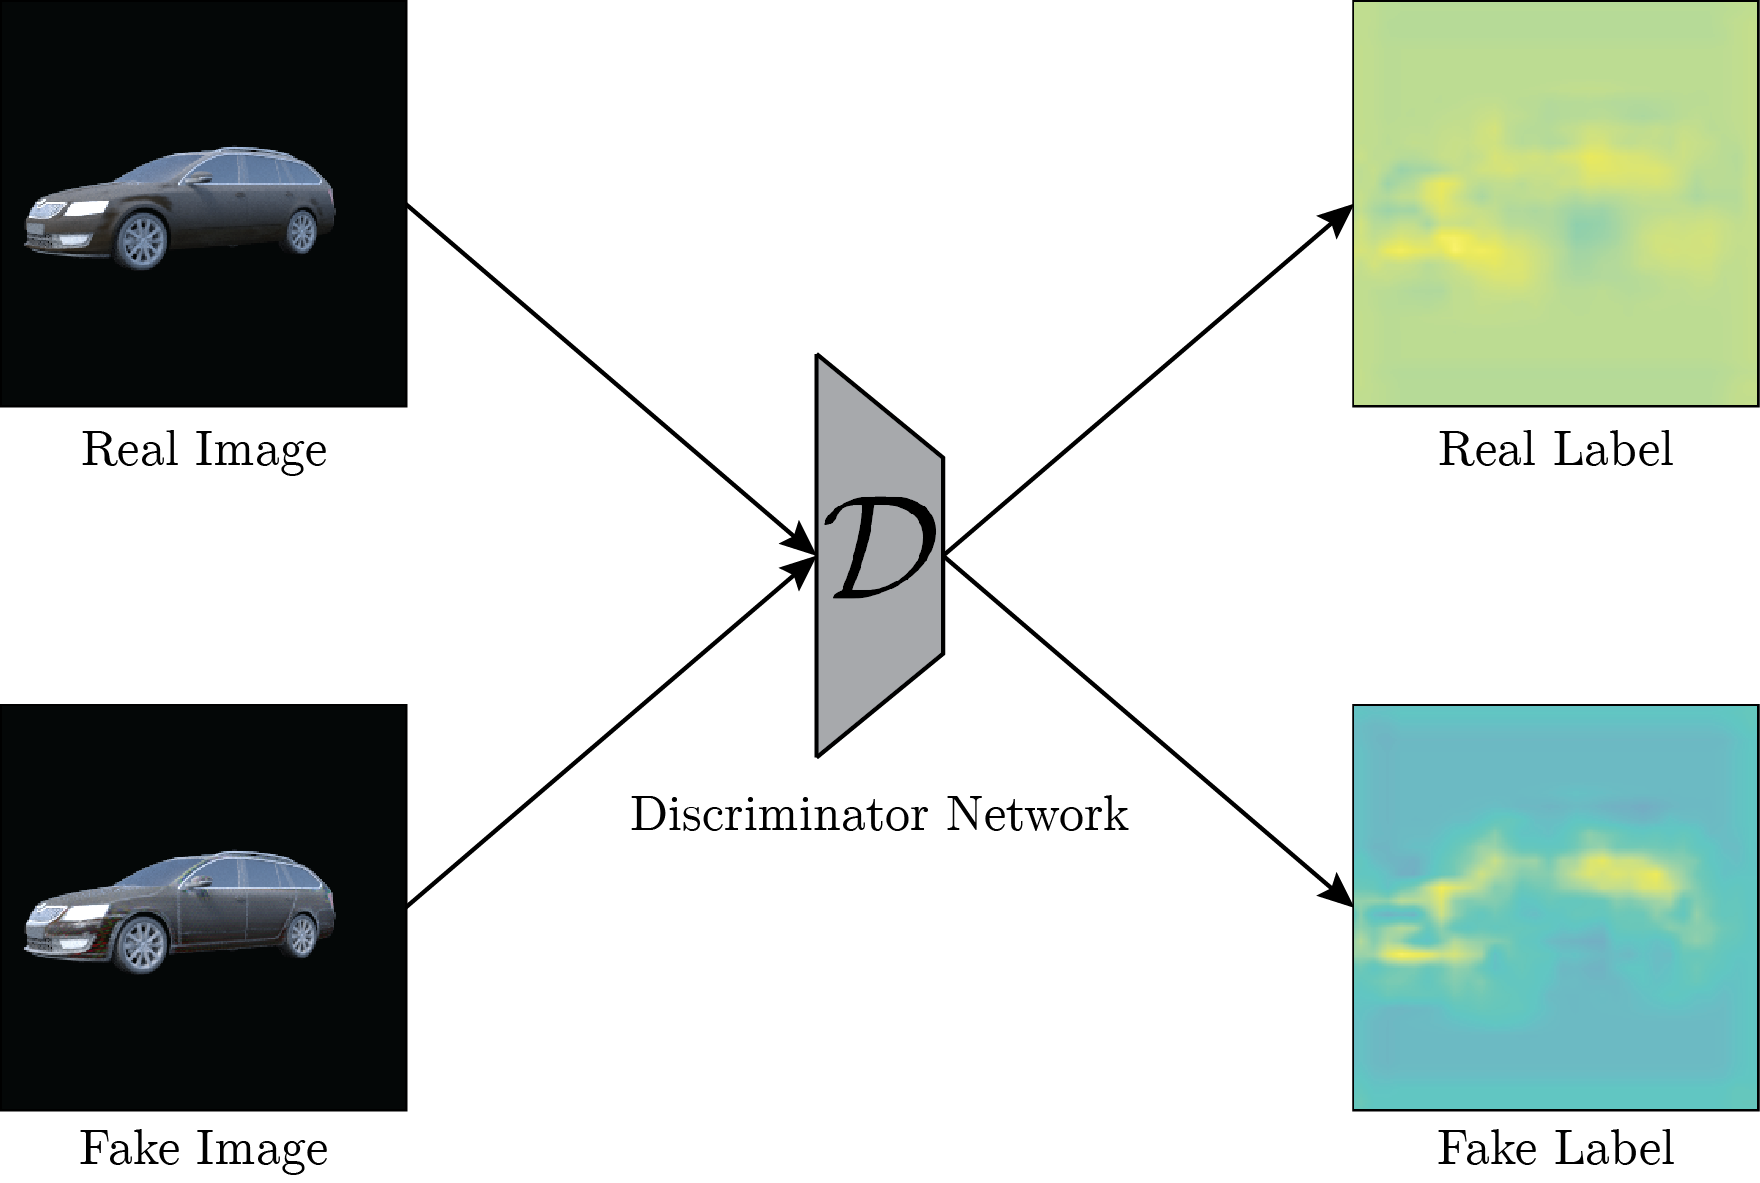
\includegraphics[width=.9\linewidth]{graphics/pipeline-2.png}
\end{figure}

\section{Differentiable Ray Tracing in Generative Models} \label{sec:diffrtgan}

The key contribution of this thesis is to frame this task as a learning problem and
incorporate the differentiable ray tracing function \cite{li2018differentiable} into the
learning process. We present a schematic of our models in Figure~\ref{fig:generator-pipeline}
and Figure ~\ref{fig:discriminator-pipeline}. We construct a convolutional neural network
$\mathcal{G}: \mathbf{x} \rightarrow \mathbf{y}$, which, given a car's surface geometry
$\mathbf{x}$, produces an albedo texture-map $\mathbf{y}$. We composit $\mathbf{y}$ onto the
base material of the car and render it using the differentiable ray tracer
$\mathcal{R}_\Phi: \mathbf{y} \rightarrow \mathbf{z}$ to obtain a rendered image $\mathbf{z}$
($\Phi$ is the parameter set which describes the scene). The combined model
$\mathcal{R}_\Phi \circ \mathcal{G}$ is fully differentiable, which allows us to train the
network weights of $\mathcal{G}$ using a loss computed from the rendered image
$\mathbf{z} = \mathcal{R}_\Phi \circ \mathcal{G}(\mathbf{x})$.

Although the render function is applicable for arbitrary network architectures, for the
scope of this thesis we train a generative adversarial network (GAN). Specifically, along with the generator $\mathcal{G}$,
our model also trains a discriminator $\mathcal{D}$ which learns to label a rendered image
of a car based on whether the albedo texture-map of the car was generated by $\mathcal{G}$
or by some ground-truth generator $\mathcal{G}_0$. $\mathcal{G}_0$ is a standard out-of-the-box
procedural surface weathering texture-map generator~\cite{bhandari2018procedural}.

\section{Model Input and Surface Parameterization}

\begin{figure}[ht]
    \centering
    \caption{The \emph{geometry buffer} is a mapping between UV-coordinates of the car
        triangle-mesh and     corresponding values of surface coordinates $\mathbf{p}$ and
        shading normals $\mathbf{n}$. We store these maps     as two RGB encoded images, with
        the three channels representing each dimension of $\mathbf{p}$ and $\mathbf{n}$
        respectively.}
    \label{fig:gbuffer}
    \vspace{0.2in}
    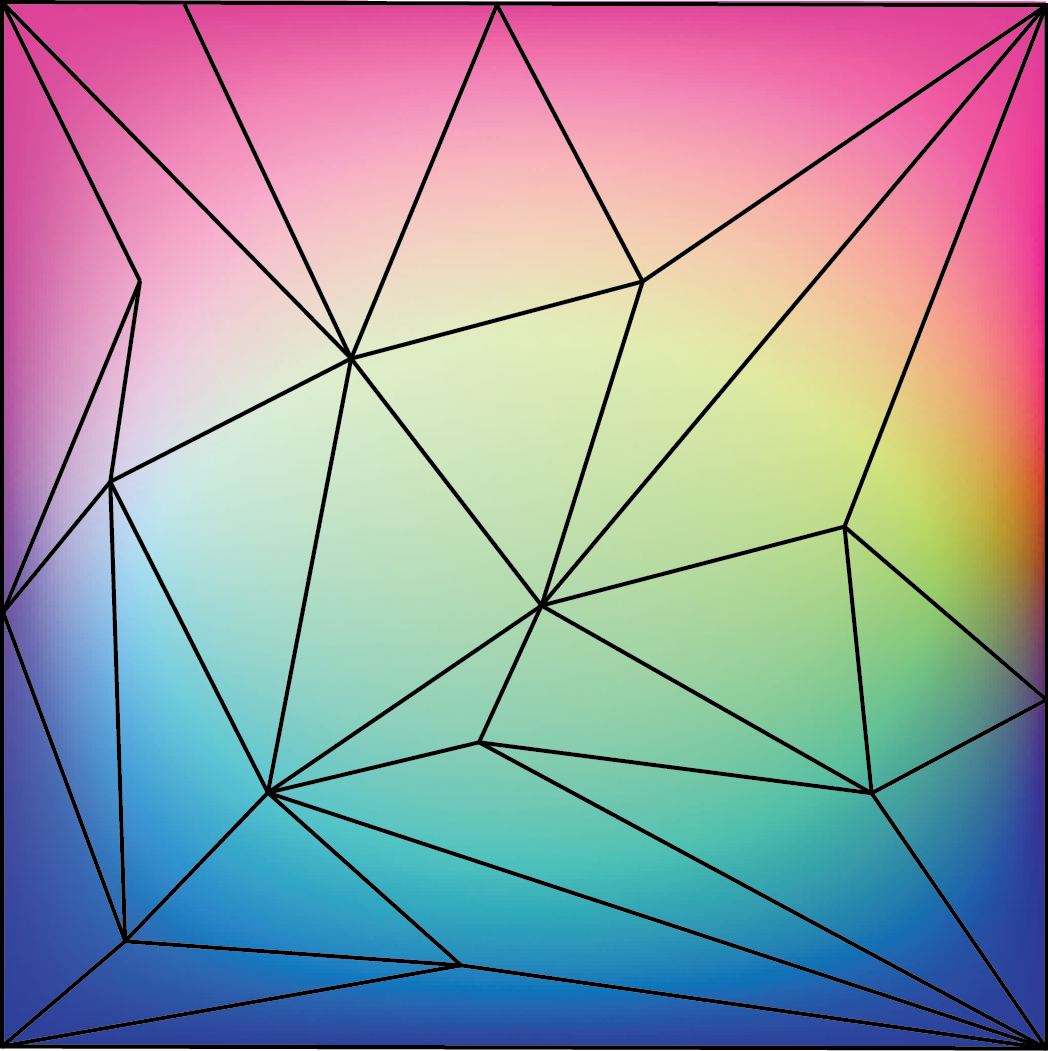
\includegraphics[width=.3\linewidth]{graphics/gbuffer.png}
\end{figure}

So far we've discussed how $\mathcal{G}$ takes as input the shape geometry of a car
$\mathbf{x}$ to produce a texture-map $\mathbf{y}$. For arbitrary generator models, the
surface geometry can be represented using any parameterization. However, in order to utilize
well tested CNN models such as \cite{johnson2016perceptual}, we require $\mathbf{x}$ to be in a
representation that is compatible with 2D convolutions.

To re-parameterize $\mathbf{x}$ into a 2D grid structure, we bake $\mathbf{x}$ onto the surface's
UV-embedding. I.e., given some UV-embededing for the input surface, for each UV-coordinate
$(u, v)$ we compute the surface's position vector $\mathbf{p}(u, v) \in \mathbb{R}^3$, and normal
vector $\mathbf{n}(u, v) \in \mathbb{R}^3$. Using $\mathbf{p}$ and $\mathbf{n}$, we form the
surface \emph{geometry buffer} $\mathbf{x} \in \mathbb{R}^6$ by concatenating the two vectors at
each UV-coordinate.

The convolutions which $\mathcal{G}$ applies to the \emph{geometry buffer} to generate the
surface albedo are similar to using 3D shape convolutions as proposed by Masci et al. 
\cite{masci2015shapenet} with the caveat of the convolution filter size changing depending on
the distortion of the UV-embedding. We provide more details about our choice of UV-embedding
as well as a discussion about desired specifications of the UV-embedding in Section
\ref{sec:uv-embedding}.